%%%%%%%%%%%%%%%%%%%%%%%%%%%%%%%%%%%%%%%%%
% Wenneker Article
% LaTeX Template
% Version 2.0 (28/2/17)
%
% This template was downloaded from:
% http://www.LaTeXTemplates.com
%
% Authors:
% Vel (vel@LaTeXTemplates.com)
% Frits Wenneker
%
% License:
% CC BY-NC-SA 3.0 (http://creativecommons.org/licenses/by-nc-sa/3.0/)
%
%%%%%%%%%%%%%%%%%%%%%%%%%%%%%%%%%%%%%%%%%

%----------------------------------------------------------------------------------------
%	PACKAGES AND OTHER DOCUMENT CONFIGURATIONS
%----------------------------------------------------------------------------------------

\documentclass[10pt, a4paper, twocolumn]{article} % 10pt font size (11 and 12 also possible), A4 paper (letterpaper for US letter) and two column layout (remove for one column)

%%%%%%%%%%%%%%%%%%%%%%%%%%%%%%%%%%%%%%%%%
% Wenneker Article
% Structure Specification File
% Version 1.0 (28/2/17)
%
% This file originates from:
% http://www.LaTeXTemplates.com
%
% Authors:
% Frits Wenneker
% Vel (vel@LaTeXTemplates.com)
%
% License:
% CC BY-NC-SA 3.0 (http://creativecommons.org/licenses/by-nc-sa/3.0/)
%
%%%%%%%%%%%%%%%%%%%%%%%%%%%%%%%%%%%%%%%%%

%----------------------------------------------------------------------------------------
%	PACKAGES AND OTHER DOCUMENT CONFIGURATIONS
%----------------------------------------------------------------------------------------

\usepackage[english]{babel} % English language hyphenation

\usepackage{microtype} % Better typography

\usepackage{amsmath,amsfonts,amsthm} % Math packages for equations

\usepackage[svgnames]{xcolor} % Enabling colors by their 'svgnames'

\usepackage[hang, small, labelfont=bf, up, textfont=it]{caption} % Custom captions under/above tables and figures

\usepackage{booktabs} % Horizontal rules in tables

\usepackage{lastpage} % Used to determine the number of pages in the document (for "Page X of Total")

\usepackage{graphicx} % Required for adding images

\usepackage{enumitem} % Required for customising lists
\setlist{noitemsep} % Remove spacing between bullet/numbered list elements

\usepackage{sectsty} % Enables custom section titles
\allsectionsfont{\usefont{OT1}{phv}{b}{n}} % Change the font of all section commands (Helvetica)

%----------------------------------------------------------------------------------------
%	MARGINS AND SPACING
%----------------------------------------------------------------------------------------

\usepackage{geometry} % Required for adjusting page dimensions

\geometry{
	top=1cm, % Top margin
	bottom=1.5cm, % Bottom margin
	left=2cm, % Left margin
	right=2cm, % Right margin
	includehead, % Include space for a header
	includefoot, % Include space for a footer
	%showframe, % Uncomment to show how the type block is set on the page
}

\setlength{\columnsep}{7mm} % Column separation width

%----------------------------------------------------------------------------------------
%	FONTS
%----------------------------------------------------------------------------------------

\usepackage[T1]{fontenc} % Output font encoding for international characters
\usepackage[utf8]{inputenc} % Required for inputting international characters

\usepackage{XCharter} % Use the XCharter font

%----------------------------------------------------------------------------------------
%	HEADERS AND FOOTERS
%----------------------------------------------------------------------------------------

\usepackage{fancyhdr} % Needed to define custom headers/footers
\pagestyle{fancy} % Enables the custom headers/footers

\renewcommand{\headrulewidth}{0.0pt} % No header rule
\renewcommand{\footrulewidth}{0.4pt} % Thin footer rule

\renewcommand{\sectionmark}[1]{\markboth{#1}{}} % Removes the section number from the header when \leftmark is used

%\nouppercase\leftmark % Add this to one of the lines below if you want a section title in the header/footer

% Headers
\lhead{} % Left header
\chead{\textit{\thetitle}} % Center header - currently printing the article title
\rhead{} % Right header

% Footers
\lfoot{} % Left footer
\cfoot{} % Center footer
\rfoot{\footnotesize Page \thepage\ of \pageref{LastPage}} % Right footer, "Page 1 of 2"

\fancypagestyle{firstpage}{ % Page style for the first page with the title
	\fancyhf{}
	\renewcommand{\footrulewidth}{0pt} % Suppress footer rule
}

%----------------------------------------------------------------------------------------
%	TITLE SECTION
%----------------------------------------------------------------------------------------

\newcommand{\authorstyle}[1]{{\large\usefont{OT1}{phv}{b}{n}\color{DarkRed}#1}} % Authors style (Helvetica)

\newcommand{\institution}[1]{{\footnotesize\usefont{OT1}{phv}{m}{sl}\color{Black}#1}} % Institutions style (Helvetica)

\usepackage{titling} % Allows custom title configuration

\newcommand{\HorRule}{\color{DarkGoldenrod}\rule{\linewidth}{1pt}} % Defines the gold horizontal rule around the title

\pretitle{
	\vspace{-30pt} % Move the entire title section up
	\HorRule\vspace{10pt} % Horizontal rule before the title
	\fontsize{32}{36}\usefont{OT1}{phv}{b}{n}\selectfont % Helvetica
	\color{DarkRed} % Text colour for the title and author(s)
}

\posttitle{\par\vskip 15pt} % Whitespace under the title

\preauthor{} % Anything that will appear before \author is printed

\postauthor{ % Anything that will appear after \author is printed
	\vspace{10pt} % Space before the rule
	\par\HorRule % Horizontal rule after the title
	\vspace{20pt} % Space after the title section
}

%----------------------------------------------------------------------------------------
%	ABSTRACT
%----------------------------------------------------------------------------------------

\usepackage{lettrine} % Package to accentuate the first letter of the text (lettrine)
\usepackage{fix-cm}	% Fixes the height of the lettrine

\newcommand{\initial}[1]{ % Defines the command and style for the lettrine
	\lettrine[lines=3,findent=4pt,nindent=0pt]{% Lettrine takes up 3 lines, the text to the right of it is indented 4pt and further indenting of lines 2+ is stopped
		\color{DarkGoldenrod}% Lettrine colour
		{#1}% The letter
	}{}%
}

\usepackage{xstring} % Required for string manipulation

\newcommand{\lettrineabstract}[1]{
	\StrLeft{#1}{1}[\firstletter] % Capture the first letter of the abstract for the lettrine
	\initial{\firstletter}\textbf{\StrGobbleLeft{#1}{1}} % Print the abstract with the first letter as a lettrine and the rest in bold
}

%----------------------------------------------------------------------------------------
%	BIBLIOGRAPHY
%----------------------------------------------------------------------------------------

\usepackage[backend=bibtex,style=authoryear,natbib=true]{biblatex} % Use the bibtex backend with the authoryear citation style (which resembles APA)

\addbibresource{example.bib} % The filename of the bibliography

\usepackage[autostyle=true]{csquotes} % Required to generate language-dependent quotes in the bibliography
 % Specifies the document structure and loads requires packages

\usepackage{hyperref} % Don't know why this has to go here, but in structure.tex does it not work for some reason

\usepackage{subcaption}
\usepackage{textcomp}

%----------------------------------------------------------------------------------------
%	ARTICLE INFORMATION
%----------------------------------------------------------------------------------------

\title{2IC80 Laboratory on Offensive Computer Security\\
	\emph{Lab Project Assignment}} % The article title

\author{
	\authorstyle{Abdel K. Bokharouss\textsuperscript{1} and Adriaan Knapen\textsuperscript{1}} % Authors
	\newline\newline % Space before institutions
	\textsuperscript{1}\institution{Eindhoven University of Technology, The Netherlands}\\ % Institution 1
}

% Example of a one line author/institution relationship
%\author{\newauthor{John Marston} \newinstitution{Universidad Nacional Autónoma de México, Mexico City, Mexico}}

\date{\today} % Add a date here if you would like one to appear underneath the title block, use \today for the current date, leave empty for no date

%----------------------------------------------------------------------------------------

\begin{document}

\maketitle % Print the title

\thispagestyle{firstpage} % Apply the page style for the first page (no headers and footers)

%----------------------------------------------------------------------------------------
%	ABSTRACT
%----------------------------------------------------------------------------------------

\lettrineabstract{fHTTP is an application which has been developed in relation to the lab assignment of the course Laboratory on Offensive Computer Security as taught at Eindhoven University of Technology. The incentive behind fHTTP is to develop (and release) an application capable of a fully-fledged ARP spoofing tool. The spoofing capabilities can then be used for other attacks which target both the confidentiality and integrity of the users and/or systems on the same (local) network. That is, we provide our users to filter traffic on the network and we facilitate the option to inject malicious code into traffic which is read, manipulated and passed on.}

In particular, we provide our users to read insecure cookies (which can be exploited for session-hijacking), to filter (unencrypted) traffic passing by based on self-specified regular-expressions and we provide our users the ability to inject code into the packets that pass by. The users can inject into an \texttt{img-}tag and the user can change the \text{accept-encoding} HTTP header to change (or disable) the content encoding algorithm. Lastly, \texttt{Nmap}-like functionality is incorporated into the application to provide the users the ability to scan the local network for potential targets. This is in relation to the \textit{main-objective} of this application: the application should be an easy-to-use tool usable in different scenarios and settings. We do not want to bother the users with continuous interaction with a command-line interface. The capabilities of the applications and a general idea of how to employ the application should be clear after one glance at \href{https://github.com/akbokha/fhttp}{\texttt{fHTTP}'s GitHub page}.

% [max 200 words] 
% Short intro describing
% - the goal of the attack
% - the impact of the attack
% - goal of the tool (simple to use)

%----------------------------------------------------------------------------------------
%	ARTICLE CONTENTS
%----------------------------------------------------------------------------------------

\section{Description of the Attack}
\label{sec:attack_desc}
The attack we implemented is aimed at intercepting HTTP cookies on a network the attacker has access to. In addition, cookies might have been set before the attack was actually started. Albeit it is required that either the cookie does not have the \emph{Secure} flag enabled or is send over an insecure connection during the attack.

A graphical representation of the attack can be seen in \autoref{fig:attack-scenario}. Below will the corresponding steps in the attack be elaborated:
\begin{enumerate}
	\item The victim connects to \texttt{S1} before the attack starts, and sets a cookie. Possibly using a secure connection.
\end{enumerate}

\noindent \emph{The attacker acquires a man-in-the-middle (MitM) position% between \texttt{Victim}, \texttt{S1} and \texttt{S2}
, for example using ARP poisoning.}
\begin{enumerate}
	\setcounter{enumi}{1}
	\item \texttt{Victim} requests a web page over HTTP to another server, since the attacker is in a MitM position will it instead be redirected to the attacker.
	\item \texttt{Attacker} redirects the request to the actual recipient in order to obtain a legitimate request.
	\item Again as a result of the MitM position will the response of the request be redirected back to the \texttt{Attacker}.
	\item The \texttt{Attacker} injects an image into the HTTP traffic with a reference to \texttt{S1} over an insecure connection.
	\item \texttt{Victim} tries to retrieve the image by sending an insecure request to \texttt{S1}, which contains the cookie set in~(1). This request is intercepted by the \texttt{Attacker} whom now has the desired cookie.
\end{enumerate}

\begin{figure}[t!]
	\centering
	\begin{subfigure}{0.4\textwidth}
	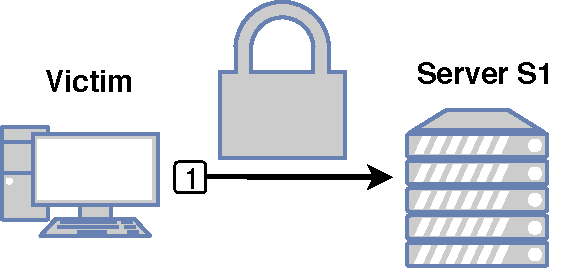
\includegraphics[width=\textwidth]{img/pre-attack}
		\caption{Before the attack.}
	\end{subfigure}

	\begin{subfigure}{0.4\textwidth}
		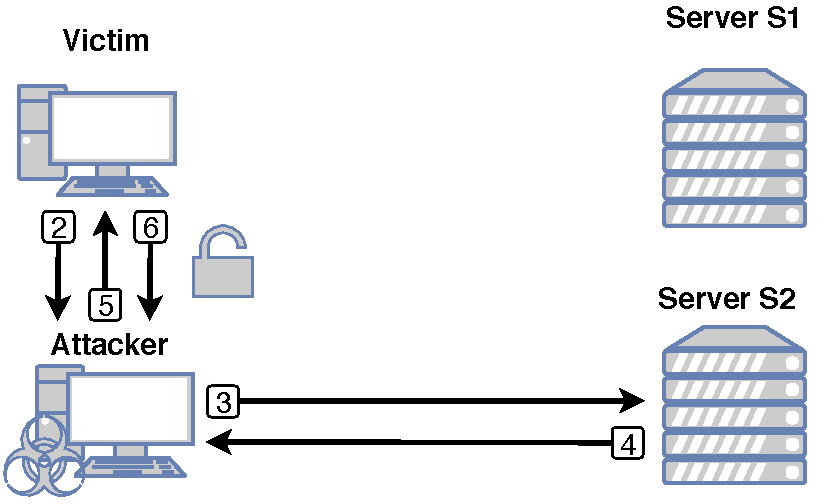
\includegraphics[width=\textwidth]{img/attack}
		\caption{During the attack.}
	\end{subfigure}
\caption{
	Graphical representation of the communication flow during the attack.}
	\label{fig:attack-scenario}
\end{figure}

An example use case of this attack could be that \texttt{S1} is the web server of an online banking service. The victim logged in earlies onto this service on a network which he or she actually trusts. Later on, the network changes and the victim does not trust the new environment enough and stops interacting with \texttt{S1}. Now the victim would expect that, without explicitly connecting to \texttt{S1}, his/her confidentiality with \texttt{S1} is untouched when interacting with other servers. Still does this attack manage to trick the victim into breaking the confidentiality, without raising any alert either by the victim or the banking service.

% [max 400 words]
% Theoretical overview on the setup of the attack, describing
% - achieving network position (MitM)
% - packet/TCP/HTTP modification

\section{Technical set-up}
\label{sec:tech_set_up}
This section is going to touch upon various technical aspects of the setup that is used to develop and test the application. In particular, the set-up which is used for the reproduction of attacks is going to be described and references to tools and other extensions that were employed to analyze the attacks are going to be given.
Initially, three virtual machines were used to reproduce the attacks and to test various aspects of the application. This is depicted in \autoref{fig:tech-set-up}. This set-up has been used to integrate ARP-spoofing and network-scanning capabilities. The local network-scanning is an integral part of the application. Since the objective is to develop an easy-to-use tool, we do not want to bother the user to find out who or what is connected to the local network. The user should be able to simply `plug-and-play' in whatever environment the application is used. This is a feature similar to the list of capabilities of tools such as \href{https://github.com/Ettercap/ettercap}{\textit{Ettercap} (a suite for man-in-the-middle attacks) } and \href{https://github.com/nmap/nmap}{\textit{Nmap} (network mapper)}. Once ARP-spoofing and local-network scans were correctly implemented and assessed to be employable in different network settings (e.g. by changing network interfaces by exploiting \texttt{ifconfig} commands: \texttt{ifconfig iface down/up}), the set-up was extended with other functionalities for different testing purposes. 

\begin{figure}[t!]
	\centering
	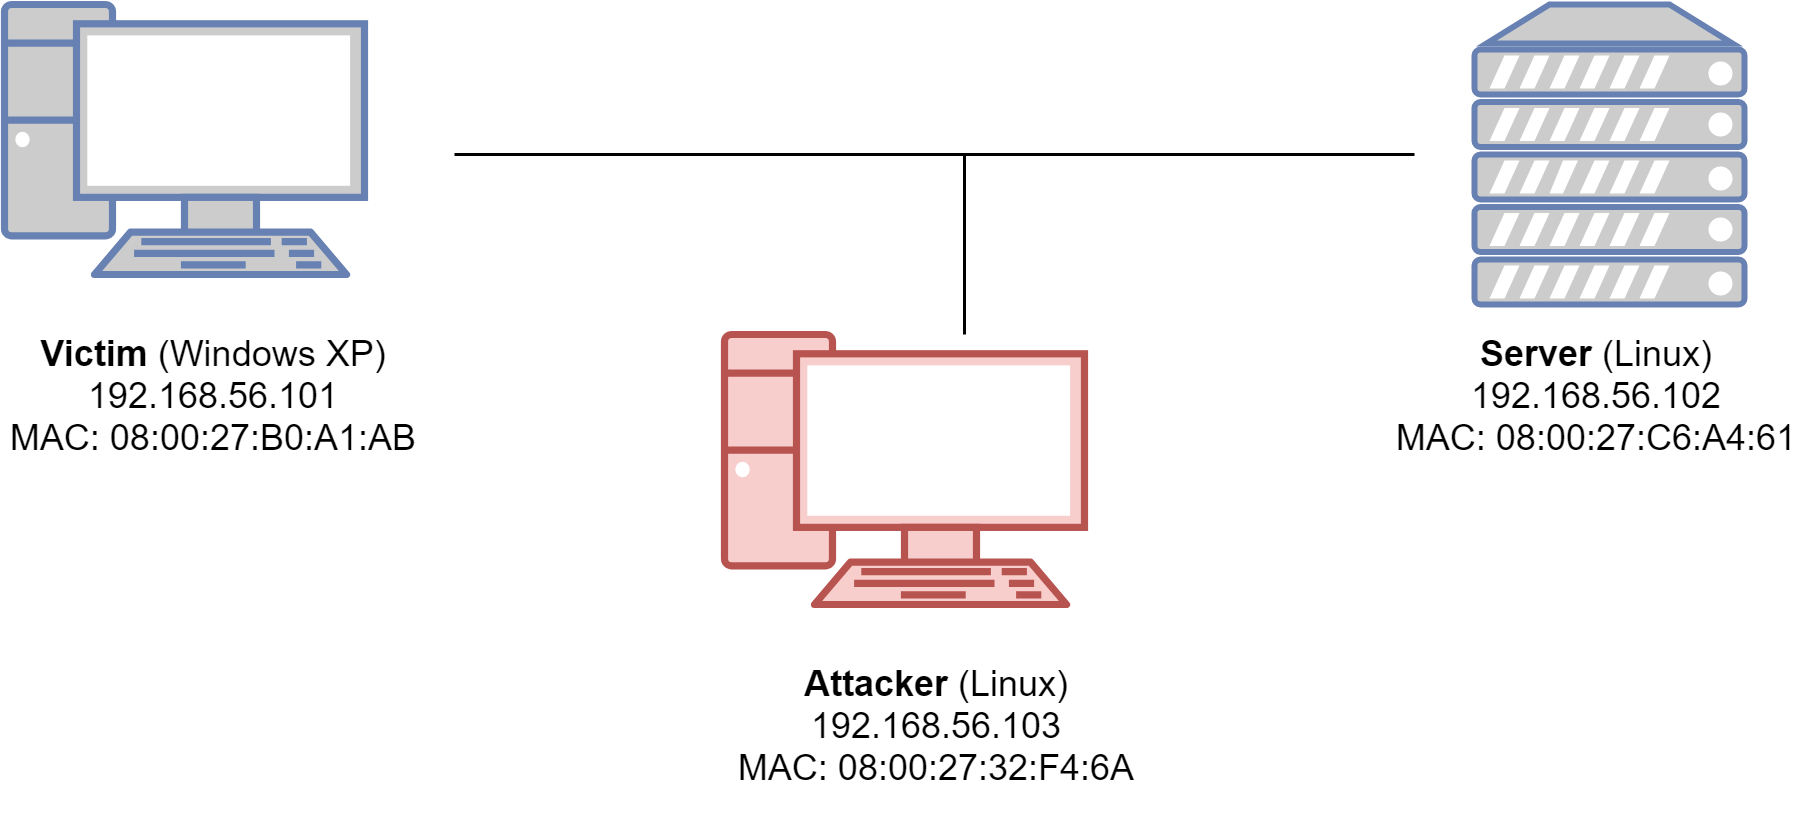
\includegraphics[width=0.4\textwidth]{img/tech_set_up.png}
	\caption{
		Set-up which is employed for application-development \& attack-reproduction and -analysis }
	\label{fig:tech-set-up}
\end{figure}

For starters, a simple web-page was hosted on the Linux server depicted on the right in \autoref{fig:tech-set-up}. This web-page has been developed to test various aspects of the applications such as the filtering of \texttt{HTTP} requests, Cookies et cetera. The dummy page is depicted in \autoref{fig:dummy_page}. One can simply set and retrieve payloads according to the tests on would like to employ.\\

\begin{figure}[h!]
	\centering
	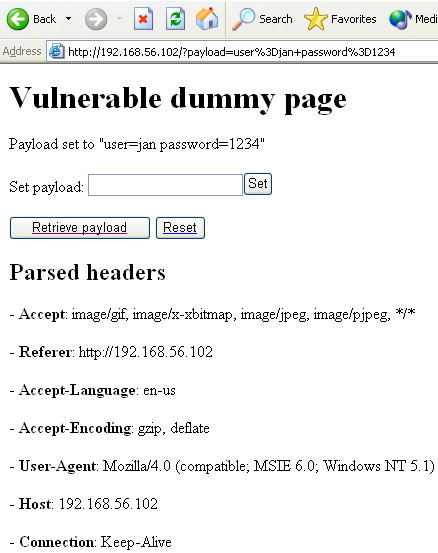
\includegraphics[width=0.5\textwidth]{img/dummy_page.png}
	\caption{
		The dummy page that was hosted on the server for testing purposes}
	\label{fig:dummy_page}
\end{figure}

Once these tests were conducted and were deemed to be successful, a fourth entity was added to the set-up depicted in \autoref{fig:dummy_page}. In particular, a second server (a copy of the first server) was added to the environment to assess the injection capabilities (e.g. \texttt{IMG-}tag injection). The victim sets a cookie in communications with this new (second) server. Subsequently, the cookie can be retrieved through an \texttt{IMG-}tag injection which contains a reference to this second server when traffic is send from the victim to the original server (as is explained in the previous section). \\

Aside from this set-up, \href{https://www.wireshark.org/}{\textit{Wireshark}} (\texttt{version: 2.2.6)} was used both in the initial development and testing phase (e.g. ARP-spoofing, local-network scan) and later phases aimed at packet modifications (e.g. injections etc.). In addition, various scripts/automated tests have been written which eased the development and testing process of the application. These tests can be found under \href{https://github.com/akbokha/fhttp/tree/master/test}{ /test/} and are (primarily) designed for the aforementioned network setting.\\

As explained before, the tool has to be easy-to-use since we both want to reach a large (tech-savvy) audience and want to showcase to less technical people how vulnerable one can be in various everyday settings by demonstrating how quick one can learn the relevant concepts (considering that we have little to no prior experience) and techniques and process them into a fully-fledged application. Hopefully, this will be a warning to them what Cyber-security researchers and engineers (or `hackers') can do when you are their `bullseye'. The afore-stated incentive behind the development of this easy-to-use application goes, therefore, hand-in-hand with the development of a graphical user-interface (GUI). Python's de-facto GUI package \href{https://wiki.python.org/moin/TkInter}{\textit{TkInter}} has, therefore, been used to develop the GUI. This does, however, introduce (yet another) dependency. The applications has been developed in- and tested with \texttt{TkInter 8.5}. In addition, \href{https://github.com/secdev/scapy}{\texttt{Scapy}} was, of course, used. The application has been extensively tested using \texttt{version: 2.3.2}. An update to \texttt{2.4.0} was considered and has been evaluated, but this affected the performance of the local network scanner. 


% [max 700 words]
% - Used tools/dependencies
% - Arp spoofing
% - Network analysis
% - accepted encoding headers
% - img tag injection
% - filtering of cookies
% [max 700 words]
% - Used tools/dependencies
% - Arp spoofing
% - Network analysis
% - accepted encoding headers
% - img tag injection
% - filtering of cookies

\section{Attack Analysis}
\label{sec:attack_analysis}
\subsection{Attack characteristics}
The attack is highly stable and reliable, it involves no probabilistic aspects - e.g. requirements to win a race condition or the like. In case the environment fulfills all requirements, then the attack is almost guaranteed to work. This is due to the fact that almost all aspects of the attack uses tricks which are also used for legitimate reasons. Hence the environment inherently supports the attack. The only exception is the modification of the HTTP payload, the obvious counter measure is using HTTPS. But the transition from the web using HTTP to HTTPS only is still ongoing, and is far from finished.

Getting into the right environment to deploy the attack will be the most challenging obstacle into employing the tool successfully. The following requirements apply:
\begin{description}
	\item[Position in the network] The attacker has to be able to achieve a MitM position in between, this could either mean that the attacker should be on the same network as the victim, or that it takes over some gateway or router which the victim uses.
	\item[Insecure cookies] The cookie which the attacker wants to intercept may not have the secure flag set, since then the browser of the victim would not include this into insecure requests. Hence making it impossible to intercept it.
	\item[HTTP traffic] The attacker needs insecure HTTP traffic in which the image tag can be injected.
\end{description}

\noindent The impact of the attack can be severe, since cookies can be extremely sensitive information like tokens of web sessions. Which, in case the web service is public, gives the attacker to take over the session and hence impersonate the victim. In practice would every online service onto which the victim logs on be an interesting target.

\subsection{Defense mechanisms}
It will be quite hard for most victims to detect or mitigate this attack, since it does not generate errors on both client and server side. The attack could either be detected by noticing the vast amount of ARP packets, although this is highly impractical for most users, since it is low level and hence requires technical knowledge in order to detect the attack. The other option is to detect the changes made to the HTTP requests, in order to make this work should the victim or server notice that either the request header or response body was tampered with. Although both are still completely legitimate according to the standards do they often contain newly introduced padding. Obviously is this not definitive proof that someone is tampering with the connection, but it does make a strong indicator.
% [max 400 words]
% Attack characteristics
% - performance (f.e. success rate)
% - environment limitations/requirements (f.e. what is required in order to achieve the MitM position)
% - impact (what could be achieved with the attack)
%
% Defense mechanisms, what could a victim do to protect them self
% - Detect the attack
% - Mitigate the attack altogether

\section{Attack Engineering}
\label{sec:attack_engineering}
% [max 300 words]
% how is the tool used, elaborate on a use case what can be achieved with the tool (mainly use screenshots?)
The easy-to-use nature of the application originates from its linear flow of instructions and capabilities. The user can, for example, not start to try to sniff packets or inject something in an \texttt{img}-tag when the ARP-cache poisoning thread has not been configured and started yet (i.e. no man-in-the-middle position). In particular, the user is lead through the following chain of exploitations, configurations and (possible) attacks: Local Network Scan $\,\to\,$ ARP Cache Poisoning $\,\to\,$ Injections and Extractions.

\begin{figure}[h!]
	\centering
	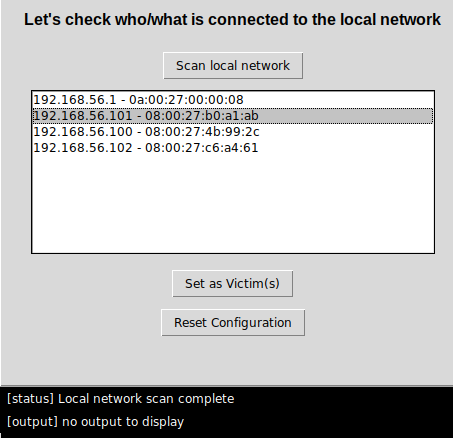
\includegraphics[width=0.5\textwidth]{img/network_scan.png}
	\caption{
		The network scan as is facilitated to the end-user}
	\label{fig:gui_network_scan}
\end{figure}

A user can perform the ARP Cache Poisoning without a local network scan (i.e. specifying the target/victim IP's himself), but execution of ARP Cache poisoning and a Local Network Scan are  preconditions for the injections and extractions. The first condition is rather trivial (mitm). The latter condition is needed to have a full map of all the IP-addresses to their respective MAC-addresses. The ARP Cache poisoning is possible on its own since it only requires the user's own mac-address (automatically retrieved in the application) and the target and victim IP'. We need to know the real mac-addresses of our victims for the injections and extractions (e.g. for packet sniffing, modification and -forwarding).\\ 

\begin{figure}[t!]
	\centering
	\begin{subfigure}{0.51\textwidth}
	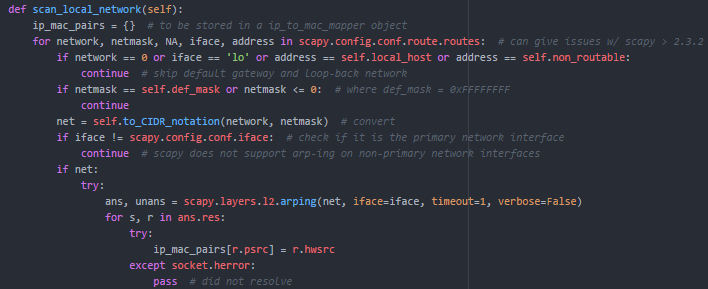
\includegraphics[width=\textwidth]{img/network_discoverer.png}
		\caption{A snippet from the source-code of the network discoverer}
	\end{subfigure}

	\begin{subfigure}{0.51\textwidth}
		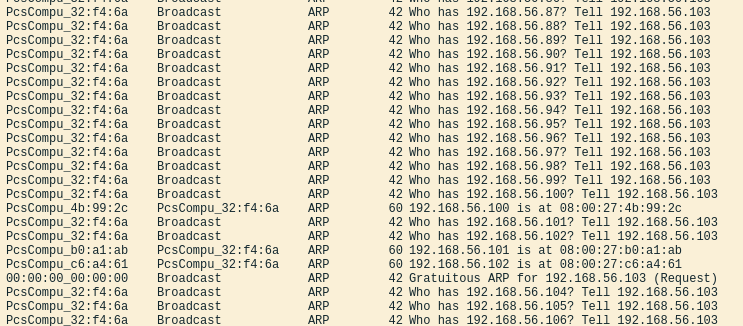
\includegraphics[width=\textwidth]{img/wireshark_network_scan}
		\caption{The ARP requests from our local network scanner in Wireshark}
	\end{subfigure}
\caption{
	Network scan in the GUI and Wireshark}
	\label{fig:network_scan}
\end{figure}

A snippet of the source code (see comments in the source code) of one of the core functionalities of our network discoverer is depicted in \autoref{fig:network_scan}. The code is rather self-explanatory. The ARP-requests can also be observed in Wireshark. This should gives you an easy to digest visualization of what is being done in the iterations of the source code (see incremental IP-addresses). The next step is the actual spoofing. If the user has selected the target and victim(s) in the list, they will be automatically loaded in the next tab \autoref{fig:arp_spoof}. ARP spoofing is done on a separate thread which keeps poisoning (10 second interval) as long the thread is alive as can be seen in the source code.\\

\begin{figure}[t!]
	\centering
	\begin{subfigure}{0.51\textwidth}
	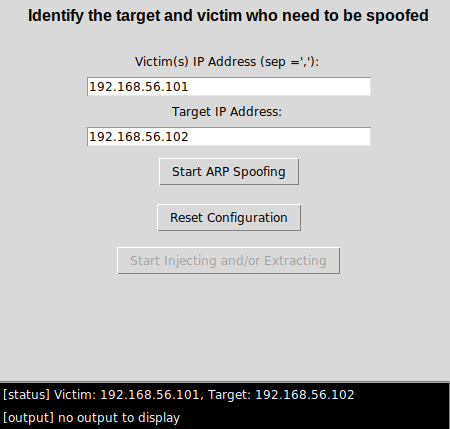
\includegraphics[width=\textwidth]{img/arp_spoofing.png}
		\caption{The ARP spoofing tab in the GUI}
	\end{subfigure}

	\begin{subfigure}{0.51\textwidth}
		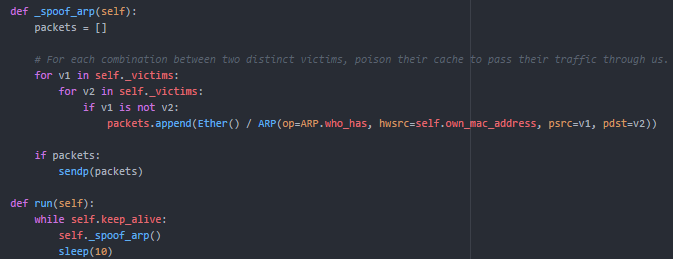
\includegraphics[width=\textwidth]{img/arp_spoof_code}
		\caption{The core functionality of the ARP-spoofing class (inherits threading.Thread)}
	\end{subfigure}
\caption{
	ARP spoofing in the GUI and source code}
	\label{fig:arp_spoof}
\end{figure}


\newpage 
Note that in the previous step the button that leads to the injection and extraction tab is still disabled. Once the `Start ARP spoofing' button is clicked one is redirected to the most fun and resourceful tab. We can see this tab in \autoref{fig:injection_filtering} where the cookie-filter has been turned on and a dummy attack has been displayed. For some extractors/filters and injectors, like the TCP regular-expression filter and \texttt{img}-tag injector, user input is needed which the user can specify in the input box that pops-up in the GUI.\\

\begin{figure}[t!]
	\centering
	\begin{subfigure}{0.45\textwidth}
	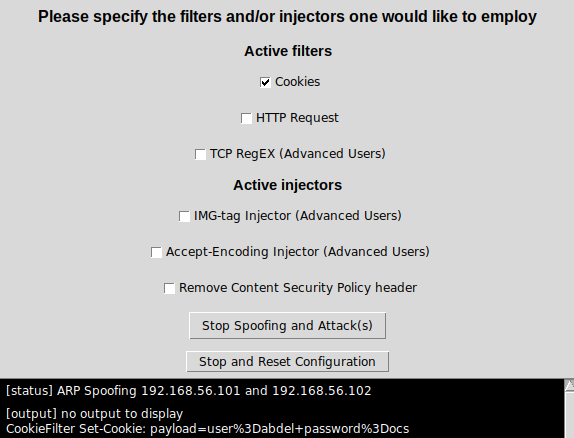
\includegraphics[width=\textwidth]{img/injection_filtering.png}
		\caption{The tab where all the injectors and filters are facilitated. Note that this is just a snippet. The output and status frame are significantly larger in the application. In addition, one can go to a previous step in the tab-navigation based GUI}
	\end{subfigure}

	\begin{subfigure}{0.45\textwidth}
		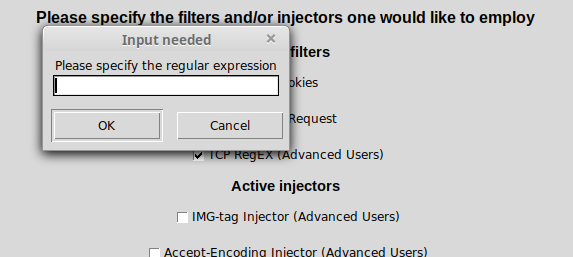
\includegraphics[width=\textwidth]{img/tcp_reg_ex.png}
		\caption{User input has to be given for some functionalities}
	\end{subfigure}
\caption{
	Extractors and Injectors}
	\label{fig:injection_filtering}
\end{figure}

The code for filters/extractors and injectors can be found in our repository (\href{https://github.com/akbokha/fhttp}{\texttt{fHTTP}'s GitHub page}). A lot emphasis and effort is put on modularity, abstraction, adhering to overall design principles and minimization of dependencies and various other (core) software engineering principles. Introducing new filters/extractors, by other contributors since it is an open-source project, is for example made easy by the facilitation of abstract classes.
% [max 300 words]
% how is the tool used, elaborate on a use case what can be achieved with the tool (mainly use screenshots?)

\newpage
\section{Discussion}
\label{sec:discussion}
\texttt{fHTTP} manages to offer a fairly easy to use tool to pull of a quite powerful attack. Still is there a lot left to improve, which mainly fall into three categories:

\begin{description}
	\item[Required technical knowledge] The graphical interface and strict flow of the application was mostly aimed at making the tool also usable for users without too much technical knowledge on networking. The current application is full of technical terms, in most cases are they irrelevant since the default values will suffice. Replacing these technical terms or explaining their consequences would be a good addition into making the tool even more easy to use.
	\item[Usability] Currently the tool only offers a method into obtaining cookies, but in most cases is this not extremely useful, since only rarely the cookie values itself are interesting. Thus the attacker would need to find a way to use this newly obtained information by itself. Hence a great addition would be a way to actually use this information, one way would be to directly load them into a browser, which would allow the attacker to use the session of the victim.
	\item[Features] The current setup of the tool would allow for many more features to be added, for now we present a tool which is mostly the minimum viable product for the attack we wanted to present. But many more aspects of the tool could be extended. Some suggestions would be different methods into obtaining the MitM position, more filters to also find other sensitive data like for example passwords, or other attacks like SSL stripping or redirecting victims to different web sites.
\end{description}

To get in conclusion, the tool offers its users everything required to successfully pull of an attack, but has even more potential for growth. The fact that the code is released open source under the MIT license allows everyone, including ourselves, to improve, to reuse, and - most importantly - to learn.
% [max 500 words]
% how could the attack be improved regarding the following aspects
% - usability
% - functionality
% - environment limitations
% - customizability
% - robustness (f.e. ensure that the attack is working)

%----------------------------------------------------------------------------------------
%	BIBLIOGRAPHY
%----------------------------------------------------------------------------------------

\printbibliography[title={Bibliography}] % Print the bibliography, section title in curly brackets

%----------------------------------------------------------------------------------------

\end{document}
